
\appendix

\section{Proofs}
\label{sec:a-proof}

\textbf{Proof of Property \ref{property_1}}

\begin{proof}
For any $\mathbf{A}' \in F(\mathbf{A})$, let $P_{\mathbf{A'}}(X | C)$ denote the distribution defined by applying Softmax on the logits given by $\mathbf{A}'$. Consider row $i$ column $j$, by definition any entry in $\mathbf{A}'$ can be expressed as $A'_{ij} = A_{ij} + \Lambda_{ii}$. It follows 
\[
P_{\mathbf{A}'}(x_j | c_i) = \frac{\exp A'_{ij}}{\sum_k \exp A'_{ik}} = \frac{\exp (A_{ij} + \Lambda_{ii})}{\sum_k \exp (A_{ik} + \Lambda_{ii})} = \frac{\exp A_{ij}}{\sum_k \exp A_{ik}} = P^*(x_j | c_i)
\]

For any $\mathbf{A}'' \in \{\mathbf{A}'' \mid \textrm{Softmax}(\mathbf{A}'') = P^* \}$, for any $i$ and $j$, we have
\[
P_{\mathbf{A}''} (x_j | c_i) = P_{\mathbf{A}} (x_j | c_i)
\]
It follows that for any $i$, $j$, and $k$,
\[
\frac{P_{\mathbf{A}''} (x_j | c_i)}{P_{\mathbf{A}''} (x_k | c_i)} = \frac{\exp A''_{ij}}{\exp A''_{ik}} = \frac{\exp A_{ij}}{\exp A_{ik}} = \frac{P_{\mathbf{A}}(x_j | c_i)}{P_{\mathbf{A}}(x_k | c_i)}
\]
As a result,
\[
A''_{ij} - A_{ij} = A''_{ik} - A_{ik}
\]
This means each row in $\mathbf{A}''$ can be obtained by adding a real number to the corresponding row in $\mathbf{A}$. Therefore, there exists a diagonal matrix $\mathbf{\Lambda} \in \mathbb{R}^{N \times N}$ such that
\[
\mathbf{A}'' = \mathbf{A} + \mathbf{\Lambda} \mathbf{J}_{N,M}
\]
It follows that $\mathbf{A}'' \in F(\mathbf{A})$.
\end{proof}

\textbf{Proof of Property \ref{property_2}}

\begin{proof}
For any $\mathbf{A}_1$ and $\mathbf{A}_2$ in $F(\mathbf{A})$, by definition we have $\mathbf{A}_1 = \mathbf{A} + \mathbf{\Lambda}_1 \mathbf{J}_{N,M}$, and $\mathbf{A}_2 = \mathbf{A} + \mathbf{\Lambda}_2 \mathbf{J}_{N,M}$ where $\mathbf{\Lambda}_1$ and $\mathbf{\Lambda}_2$ are two diagonal matrices. It can be rewritten as
\[
\mathbf{A}_1 = \mathbf{A}_2 + (\mathbf{\Lambda}_1 - \mathbf{\Lambda}_2) \mathbf{J}_{N,M}
\]
Let $S$ be a maximum set of linearly independent rows in $\mathbf{A}_2$. Let $\mathbf{e}_N$ be an all-ones vector with dimension $N$. The $i$-th row vector $\mathbf{a}_{1,i}$ in $\mathbf{A}_1$ can be written as
\[
\mathbf{a}_{1,i} = \mathbf{a}_{2,i} + (\Lambda_{1,ii} - \Lambda_{2,ii}) \mathbf{e}_N
\]
Because $\mathbf{a}_{2,i}$ is a linear combination of vectors in $S$, $\mathbf{a}_{1,i}$ is a linear combination of vectors in $S \cup \{\mathbf{e}_N\}$. It follows that
\[
\text{rank}(\mathbf{A}_1) \leq \text{rank}(\mathbf{A}_2) + 1
\]

Similarly, we can derive
\[
\text{rank}(\mathbf{A}_2) \leq \text{rank}(\mathbf{A}_1) + 1
\]

Therefore,
\[
|\text{rank}(\mathbf{A}_1) - \text{rank}(\mathbf{A}_2)| \leq 1
\]
\end{proof}

\textbf{Proof of Proposition \ref{prop}}

\begin{proof}
If there exists a parameter $\theta$ such that $P_\theta(X | c) = P^*(X | c)$ for all $c$ in $\mathcal{L}$, by Lemma \ref{lemma}, we have $\mathbf{H}_\theta \mathbf{W}_\theta^\top \in F(\mathbf{A})$. As a result, there exists a matrix $\mathbf{A}' \in F(\mathbf{A})$ such that $\mathbf{H}_\theta \mathbf{W}_\theta^\top = \mathbf{A}'$. Because $\mathbf{H}_\theta$ and $\mathbf{W}_\theta$ are of dimensions $(N \times d)$ and $(M \times d)$ respectively, we have
\[
d \geq \text{rank}(\mathbf{A}') \geq \min_{\mathbf{A''} \in F(\mathbf{A})} \text{rank}(\mathbf{A}'')
\]


If $d \geq \min_{\mathbf{A''} \in F(\mathbf{A})} \text{rank}(\mathbf{A}'')$, there exist matrices $\mathbf{A}' \in F(\mathbf{A})$, $\mathbf{H}' \in \mathbb{R}^{N \times d}$ and $\mathbf{W}' \in \mathbb{R}^{M \times d}$, such that $\mathbf{A}'$ can be factorized as $\mathbf{A}' = \mathbf{H}' \mathbf{W}'^\top$. Because $\mathcal{U}$ is a universal approximator, there exists $\theta$ such that $\mathbf{H}_\theta = \mathbf{H}'$ and $\mathbf{W}_\theta = \mathbf{W}'$. By Lemma \ref{lemma}, $P_\theta(X | c) = P^*(X | c)$ for all $c$ in $\mathcal{L}$.
\end{proof}

\section{Experiment setting and Hyper-parameters}
\subsection{PTB and WT2}
\label{sec:a-exp-sota}
The hyper-parameters used for MoS in language modeling experiment is summarized below.
\begin{table*}[!h]
	\small
	\centering
	\begin{tabular}{l|ccc }
		\toprule
		\bf Hyper-parameter & \bf PTB & \bf WT2 \\ 
		\midrule
		Learning rate & 20 & 15 & \\
		Batch size & 12 & 15 & \\
		Embedding size & 280 & 300 \\ 
		RNN hidden sizes & [960, 960, 620] & [1150,1150,650] \\
		Number of mixture components & 15 & 15 \\
		\midrule
		Word-level V-dropout & 0.10 & 0.10 \\
		Embedding V-dropout & 0.55 & 0.40 \\
		Hidden state V-dropout & 0.20 & 0.225\\
		Recurrent weight dropout~\citep{wan2013regularization} & 0.50 & 0.50 \\
		Context vector V-dropout & 0.30 & 0.30 \\
		\bottomrule
	\end{tabular}
	\caption{\small
		Hyper-parameters used for MoS. V-dropout abbreviates variational dropout~\citep{gal2016theoretically}. See \citep{merity2017regularizing} for more detailed descriptions.
	}
	\label{table:hyper-sota-train}
	\vspace{-1em}
\end{table*}

The hyper-parameters used for dynamic evaluation of MoS is summarized below.
\begin{table*}[!h]
	\small
	\centering
	\begin{tabular}{l|ccc }
		\toprule
		\bf Hyper-parameter & \bf PTB & \bf WT2 \\ 
		Batch size & 100 & 100\\
		learning rate ($\eta$) & 0.002 & 0.002 \\
		$\epsilon$ &0.001 & 0.002 \\
		$\lambda$ &0.075 & 0.02 \\
		\bottomrule
	\end{tabular}
	\caption{\small
		Hyper-parameters used for dynamic evaluation of MoS. See \citep{krause2017dynamic} for more detailed descriptions.
	}
	\label{table:hyper-sota-dyeval}
	\vspace{-1em}
\end{table*}

\subsection{1B Word Dataset}
\label{sec:a-exp-1b}

%In the 1/10 training data setting, we pick 10 shards from the total 100 training shards, which are specifically \texttt{[train-01, train-11, \dots, train-81, train-91]}. 
For training, we use all of the 100 training shards.
For validation, we use two shards from the heldout set, namely \texttt{[heldout-00, heldout-10]}. 
For test, we use another three shards from the heldout set, namely \texttt{[heldout-20, heldout-30, heldout-40]}. 

The hyper-parameters are listed below.
\begin{table*}[!h]
	\small
	\centering
	\begin{tabular}{l|ccc }
		\toprule
		\bf Hyper-parameter & \bf Softmax & \bf MoS-7 \\
		\midrule
		Learning rate & 20 & 20 & \\
		Batch size & 60 & 60 & \\
		BPTT langth & 35 & 35 & \\
		Embedding size & 1024 & 900 \\ 
		RNN hidden sizes & [1024, 1024] & [1024,1024] \\
		Dropout rate & 0 & 0 \\
		\bottomrule
	\end{tabular}
	\caption{\small
		Hyper-parameters used for Softmax and MoS in experiment on 1B word dataset.
	}
	\label{table:hyper-1b}
	\vspace{-1em}
\end{table*}


\section{Additional experiments}

\subsection{Higher empirical rank of  MoS compared to MoC and Softmax}
\label{sec:a-rank}
\begin{figure}[!h]
	\centering
	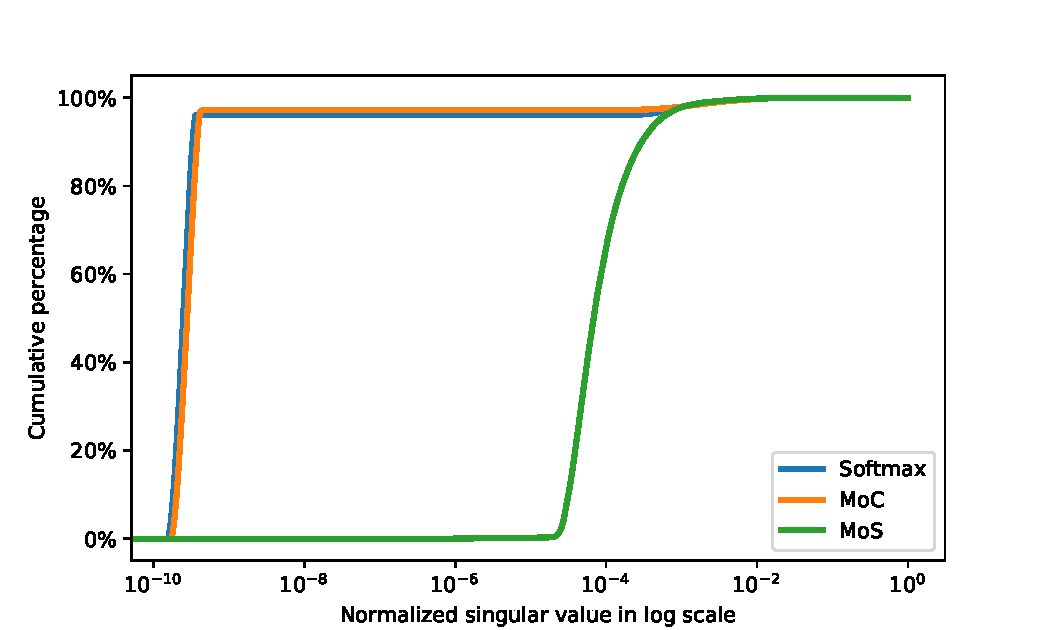
\includegraphics[width=0.8\linewidth]{FIG/singular-all.pdf}
	\captionof{figure}{\small Cumulative percentage of normalized singulars given a value in $[0, 1]$.}
	\label{fig:quantitative}
\end{figure}
In section \ref{sec:exp}, we compute the rank of different models based on the non-zero singular values of the empirical log-likelihood matrix.
Since there can be roundoff mistakes, a less error-prone approach is to directly study the distribution of singular values.
Specifically, if more singular values have relatively larger magnitude, the rank of the matrix tends to be higher.
Motivated from this intuition, we visualize the distribution of the singular values. To account for the different magnitudes of singular values from different models, we first normalize all singular values to $[0, 1]$. Then, we plot the cumulative percentage of normalized singular values, i.e., percentage of normalized singular values below a threshold, in Figure \ref{fig:quantitative}. As we can see, most of the singular values of Softmax and MoC concentrate on an area with very low values. In comparison, the concentration area of the MoS singular values is not only several orders larger, but also spans a much wider region. 
Intuitively, MoS utilizes the corresponding singular vectors to capture a larger and more diverse set of contexts. 

\begin{table}[!h]
	\centering
	\small
	\begin{tabular}{l|cc}
		\toprule
		\bf Model & \bf Validation & \bf Test \\
		\midrule
		Softmax & 4.869 & 4.763  \\
		MoC & 4.955 & 4.864 \\
		MoS & \bf 5.400 & \bf 5.284 \\
		\bottomrule
	\end{tabular}
	\caption{Empirical expected pairwise KLD on PTB.}
	\label{table:kld}
\end{table}

What's more, another indicator of high rank is that the model can precisely capture the nuance of difference contexts.
If a model can better capture the distinctions among contexts, we expect the next-step conditional distributions to be less similar to each on average. Based on this intuition, we use the expected pairwise Kullback–Leibler divergence (KLD), i.e., $\mathbb{E}_{c, c' \sim \mathcal{C}} \left[ \mathrm{KLD}(P(X \mid c) \| P(X \mid c')) \right]$ where $\mathcal{C}$ denotes all possible contexts, as another metric to evaluate the ranks of the three models (MoS, MoC and Softmax). Practically, we sample $c, c'$ from validation or test data of PTB to get the empirical estimations for the three models, which are shown in the right half of Table \ref{table:kld}. As we expected, MoS achieves higher expected pairwise KLD, indicating its superiority in covering more contexts of the next-token distribution.

\subsection{An inverse experiment on character-level language modeling}
\label{sec:a-charlm}
\begin{table}[!h]
	\centering
	\small
%	\begin{minipage}[b]{0.55\linewidth}
%		\small
%		\centering
		\begin{tabular}{ll|c|ccc}
			\toprule
			\bf Model && \bf \#Param & \bf Train & \bf Validation & \bf Test \\
			\midrule
			Softmax &(hid1024, emb1024) & 8.42M & 1.35 & 1.41 & 1.49 \\
			MoS-7    &(hid910, emb510)     & 8.45M & 1.35 & 1.40 & 1.49 \\
			MoS-7    &(hid750, emb750)    & 8.45M & 1.38 & 1.42 & 1.50 \\
			MoS-10  &(hid860, emb452)    & 8.43M & 1.35 & 1.41 & 1.49 \\
			MoS-10  &(hid683, emb683)    & 8.43M & 1.38 & 1.42 & 1.50 \\
			\bottomrule
		\end{tabular}
		\caption{\small BPC comparison on text8. For MoS, ``-$n$'' indicates using $n$ mixtures. ``hid'' and ``emb'' denote the hidden size and embedding size respectively.}
		\label{table:charlm}
\end{table}
Here, we detail the inverse experiment, which shows that when Softmax does \textit{not} suffer from a rank limitation, using MoS will \textit{not} improve the performance.
Notice that character-level language modeling (CharLM) is exactly such a problem, because the rank of the log-likelihood matrix is upper bounded by the vocabulary size, and CharLM usually has a very limited vocabulary (tens of characters).
In this case, with the embedding size being hundreds in practice, Softmax is no longer a bottleneck in this task. 
Hence, we expect MoS to yield similar performance to Softmax on CharLM.

We conduct experiments of CharLM using the text8 dataset~\citep{mahoney2011large}, which consists of 100M characters including only alphabetical characters and spaces derived from Wikipedia. We follow \citet{mikolov2012subword} and use the first 90M characters for training, the next 5M for validation and the final 5M for testing.
The standard evaluation metric bit-per-character (BPC) is employed.
We employ a 1-layer 1024-unit LSTM followed by Softmax as the baseline. For MoS, we consider 7 or 10 mixtures and reduce the hidden and/or embedding size to match the baseline capacity. When decreasing the hidden and/or embedding size, we either keep both the same, or make the hidden size relatively larger. 
The results are summarized in Table \ref{table:charlm}. Clearly, the Softmax and MoS obtain the same BPC on the test set and comparable BPC on the validation set, which well match our hypothesis.
Since the only difference in word-level language modeling is the existence of the Softmax bottleneck, the distinct behavior of MoS again supports our hypothesis that it is solving the Softmax bottleneck problem.

\subsection{MoS Computational Time}
\label{sec:a-time}
\begin{table}[!h]
	\small
	\centering
	\begin{tabular}{l|rrrrrrrr}
		\toprule
		% \bf Model & \multicolumn{1}{c}{\bf PTB/bs} & \multicolumn{1}{c}{\bf WT2} \\
		\bf Model & PTB/bs & PTB/best-1 & WT2/bs & WT2/best-1 & WT2/best-3 & 1B/bs & 1B/best-1 & 1B/best-3 \\
		\midrule
		Softmax & 1x   & 1x	  	& 1x	&1x		&1x		&1x		&1x		&1x\\
		MoS-5   & 1.2x & --	 	& 1.3x	&--		&--		&--		&--		&--\\
		MoS-7	& --   & --		& --	&--		&--		&3.8x	&5.7x	&2.1x\\
		MoS-10  & 1.6x & --		& 1.9x	&--		&--		&--		&--		&--\\
		MoS-15  & 1.9x & 2.8x	& 2.5x	&6.4x	&2.9x	&--		&--		&--\\
		\bottomrule
	\end{tabular}
	\caption{\small Training time slowdown compared to Softmax. MoS-$K$ means using $K$ mixture components. ``bs'' indicates Softmax and MoS use the same batch sizes on one GPU. ``best-1'' and ``best-3'' refer to the settings where Softmax and MoS obtain their own best perplexity, with 1 and 3 GPUs respectively.}
	\label{table:walltime}
\end{table}

We evaluate the additional computational cost introduced by MoS. We consider two sets of controlled experiments. In the first set, we compare the training time of MoS and Softmax using the same batch sizes. In the second set, we compare the training time of two methods using the hyper-parameter settings that achieve the best performance for each model (i.e., the settings in Tables \ref{table:PTB}, \ref{table:WT2}, and \ref{table:1bword}). In both sets, we control two models to have comparable model sizes.

The results on the three datasets are shown in Table \ref{table:walltime}. Thanks to the efficiency of matrix multiplication on GPU, the computational wall time of MoS is actually sub-linear w.r.t. the number of Softmaxes $K$. In most settings, we observe a two to three times slowdown when using MoS. Specifically, the ``bs'' setting measures the computational cost introduced by MoS given enough memory, which is 1.9x, 2.5x, and 3.8x slowdown on PTB, WT2, and 1B respectively. The ``best-1'' setting is usually slower compared to ``bs'', because a single batch does not fit into the memory of a single GPU using MoS, in which case we have to split one batch into multiple small ones, resulting in further slowdown. In this sense, the gap between ``best-1'' and ``bs'' measures the computational cost introduced due to the increase of memory consumed by MoS. 
The ``best-3'' alleviates this issue by using three GPUs, which allows larger-batch training for MoS. In this case, we reduce the computational cost to 2.9x on WT2 and 2.1x on 1B with our best performing model.

Note that the computational cost is closely related to the batch size, which is interleaved with optimization. Though how batch sizes affect optimization remains an open question and might be task dependent, we believe the ``best-1'' and ``best-3'' settings well reflect the actual computational cost brought by MoS on language modeling tasks.

 \subsection{Qualitative Analysis}
 \label{sec:a-qualitative} 
 Since MoC shows a stronger performance than Softmax on PTB, the qualitative study focuses on the comparison between MoC and MoS. Concretely, given the same context (previous tokens), we search for prediction steps where MoS achieves lower negative log loss than MoC by a margin. We show some representative cases in Table \ref{table:qualitative} with the following observations:
 \begin{table*}[t]%[!h]
 	\centering
 	\footnotesize
 	\begin{tabular}{l*{5}{C}}
 		\toprule
 		%%%%%% 1st
 		{\bf \#1 Context}
 		&\multicolumn{5}{p{\contextlength}}{managed properly and with a long-term outlook these can become investment-grade quality properties <eos> canadian <unk> production totaled N metric tons in the week ended oct. N up N N from the preceding week 's total of N \blank} \\
 		\midrule
 		{\bf MoS top-5} 
 		&million 0.38& \textbf{tons 0.24}& billion 0.09& barrels 0.06& ounces 0.04 \\
 		\midrule
 		{\bf MoC top-5} 
 		&billion 0.39& million 0.36& trillion 0.05& <eos> 0.04& N 0.03 \\
 		\midrule
 		{\bf Reference} 
 		&\multicolumn{5}{p{\contextlength}}{canadian <unk> production totaled N metric tons in the week ended oct. N up N N from the preceding week 's total of N \underline{ \textbf{tons} } statistics canada a federal agency said <eos>} \\
 		\midrule\midrule
 		%%%%%% 2nd
 		{\bf \#2 Context}
 		&\multicolumn{5}{p{\contextlength}}{the thriving <unk> street area offers <unk> of about \$ N a square foot as do <unk> locations along lower fifth avenue <eos> by contrast <unk> in the best retail locations in boston san francisco and chicago rarely top \$ N \blank} \\
 		\midrule
 		{\bf MoS top-5} 
 		&<eos> 0.36& \textbf{a 0.13}& to 0.07& for 0.07& and 0.06 \\
 		\midrule
 		{\bf MoC top-5} 
 		&million 0.39& billion 0.36& <eos> 0.05& to 0.04& of 0.03 \\
 		\midrule
 		{\bf Reference} 
 		&\multicolumn{5}{p{\contextlength}}{by contrast <unk> in the best retail locations in boston san francisco and chicago rarely top \$ N \underline{ \textbf{a} } square foot <eos>} \\
 		\midrule\midrule
 		%%%%%% 3rd
 		{\bf \#3 Context}
 		&\multicolumn{5}{p{\contextlength}}{as other <unk> governments particularly poland and the soviet union have recently discovered initial steps to open up society can create a momentum for radical change that becomes difficult if not impossible to control <eos> as the days go by the south \blank} \\
 		\midrule
 		{\bf MoS top-5} 
 		&africa 0.15& \textbf{african 0.15}& <eos> 0.14& korea 0.08& korean 0.05 \\
 		\midrule
 		{\bf MoC top-5} 
 		&<eos> 0.38& and 0.08& of 0.06& or 0.05& <unk> 0.04 \\
 		\midrule
 		{\bf Reference} 
 		&\multicolumn{5}{p{\contextlength}}{as the days go by the south \underline{ \textbf{african} } government will be ever more hard pressed to justify the continued <unk> of mr. <unk> as well as the continued banning of the anc and enforcement of the state of emergency <eos>} \\ 
 		\midrule\midrule
 		%%%%%% 4th
 		{\bf \#4 Context}
 		&\multicolumn{5}{p{\contextlength}}{shares of ual the parent of united airlines were extremely active all day friday reacting to news and rumors about the proposed \$ N billion buy-out of the airline by an <unk> group <eos> wall street 's takeover-stock speculators or risk arbitragers had placed unusually large bets that a takeover would succeed and \blank} \\
 		\midrule
 		{\bf MoS top-5} 
 		&the 0.14& that 0.07& \textbf{ual 0.07}& <unk> 0.03& it 0.02 \\
 		\midrule
 		{\bf MoC top-5} 
 		&the 0.10& <unk> 0.06& that 0.05& in 0.02& it 0.02 \\
 		\midrule
 		{\bf Reference} 
 		&\multicolumn{5}{p{\contextlength}}{wall street 's takeover-stock speculators or risk arbitragers had placed unusually large bets that a takeover would succeed and \underline{ \textbf{ual} } stock would rise <eos>} \\ 
 		\midrule\midrule
 		%%%%%% 5th
 		{\bf \#5 Context}
 		&\multicolumn{5}{p{\contextlength}}{the government is watching closely to see if their presence in the <unk> leads to increased <unk> protests and violence if it does pretoria will use this as a reason to keep mr. <unk> behind bars <eos> pretoria has n't forgotten why they were all sentenced to life <unk> in the first place for sabotage and \blank} \\
 		\midrule
 		{\bf MoS top-5} 
 		&<unk> 0.47& violence 0.11& \textbf{conspiracy 0.03}& incest 0.03& civil 0.03 \\
 		\midrule
 		{\bf MoC top-5} 
 		&<unk> 0.41& the 0.03& a 0.02& other 0.02& in 0.01 \\
 		\midrule
 		{\bf Reference} 
 		&\multicolumn{5}{p{\contextlength}}{pretoria has n't forgotten why they were all sentenced to life <unk> in the first place for sabotage and \underline{ \textbf{conspiracy} } to <unk> the government <eos>} \\
 		\midrule\midrule
 		%%%%%% 6th
 		{\bf \#6 Context}
 		&\multicolumn{5}{p{\contextlength}}{china 's <unk> <unk> program has achieved some successes in <unk> runaway economic growth and stabilizing prices but has failed to eliminate serious defects in state planning and an <unk> drain on state budgets <eos> the official china daily said retail prices of <unk> foods have n't risen since last december but acknowledged that huge government \blank} \\ 
 		\midrule
 		{\bf MoS top-5} 
 		&\textbf{subsidies 0.15}& spending 0.08& officials 0.04& costs 0.04& <unk> 0.03  \\
 		\midrule
 		{\bf MoC top-5} 
 		&officials 0.04& figures 0.03& efforts 0.03& <unk> 0.03& costs 0.03 \\
 		\midrule
 		{\bf Reference} 
 		&\multicolumn{5}{p{\contextlength}}{the official china daily said retail prices of <unk> foods have n't risen since last december but acknowledged that huge government \underline{ \textbf{subsidies} } were a main factor in keeping prices down <eos>} \\
 		\bottomrule
 	\end{tabular}
 	\caption{\small
 		Compaison of next-token prediction on Penn Treebank test data. N stands for a number as the result of preprocessing~\citep{mikolov2010recurrent}. The context shown only includes the previous sentence and the current sentence the prediction step resides in.
 	}
 	\label{table:qualitative}
 \end{table*}
 \begin{itemize}[leftmargin=1.5em,label=$\bullet$]
 	\item Comparing the first two cases, given the same preceding word ``N'', MoS flexibly adjusts its top predictions based on the different topic quantities being discussed in the context. In comparison, MoC emits quite similar top choices regardless of the context, suggesting its inferiority in make context-dependent predictions.
 	\item In the 3rd case, the context is about international politics, where country/region names are likely to appear. MoS captures this nuance well, and yields top choices that can be used to complete a country name given the immediate preceding word ``south''. Similarly, in the 4th case, MoS is able to include ``ual'', a core entity of discussion in the context, in its top predictions.
 	In contrast, MoC gives rather generic predictions irrieselevant to the context in both cases. 
 	\item For the 5th and the 6th example, we see MoS is able to exploit less common words accurately according to the context, while MoC fails to yield such choices. This well matches our analysis that MoS has the capacity of modeling context-dependent language.
 \end{itemize}
 